\section{Introduction}

Exoskeletons are robotic interfaces for human-robot interaction where the highest physical symbiosis with the human operator is achieved 
\cite{Frisoli2019Encylopedia}.
%\hldoing{insert here wearable robots citation from encylopedia of robotics}
Unlike many industrial robots  designed to exhibit a stiff structure and behavior,  therefore to be used with a rigid position control, the exoskeletons are in direct contact with humans, so that  they have to satisfy  safety and compliance requirements common to physical Human-Robot Interaction (pHRI) devices \cite{bajcsy2017learning}.
\par In physical Human-Robot Interaction applications, moreover  there are other performance measures inherently depending on the actuation and control that need to be considered, among which the two most relevant ones are {\em transparency} and  {\em haptic rendering}: 

%
%\begin{description}[\setlabelwidth{$\alpha\omega\pi\theta\mu$}\usemathlabelsep]
%	\item[$\gamma\delta\beta$] Is the index of..
%	\item[$\alpha\omega\pi\theta\mu$] Gives the....
%\end{description}
	
%	[\setlabelwidth{Haptic rendering}]
\noindent
%\setlength{\IEEEdlabelindent}{-0.5 \parindent}
\setlength{\IEEEiednormlabelsep}{-2 \parindent}
\begin{IEEEdescription}
	%[\IEEEsetlabelwidth{Very long label} \IEEEusemathlabelsep]
	\item[{\bf Transparency }] \hspace{2 cm}
	%Transparency
	 relates to the ability of the
	robotic system interacting with a human who is moving
	voluntarily
	not to apply any assistance/
	resistance to free motion
	\cite{jarrasse2010methodology},
	or equivalently means that the robot’s
	reaction forces perceived by the user are minimal \cite{just2018exoskeleton}.
	No standard procedures exist for the measurement of transparency in pHRI, but for exoskeletons there is a general consensus  to refer not only to end-effector resistance forces, but also to single joints resistance torques or measurements at contact points \cite{just2018exoskeleton}.
	\item[{\bf Haptic rendering} ] %\hspace{2 cm}
	 %Haptic rendering 
	 \hspace{2.7 cm}
	  refers to the capability of the device to render a desired dynamic behavior, such as a virtual impedance  or a virtual wall, i.e. a
	task featuring both very high impedance (when in contact
	with the wall) and very low impedance (when out of
	contact) \cite{colgate1994factors}. Better mechanical structures,
	including appropriate dimensioning of the sensors and
	actuators, combined with more effective
	control strategies  should predict the maximum
	stiffness that can be displayed by existing devices   \cite{diolaiti2005criterion}.
\end{IEEEdescription}


In the last two decades, several exoskeleton solutions have been proposed using different implementation principles according to the field of application, such as  neurorehabilitation and assistance \cite{lo2012exoskeleton,pirondini2016evaluation,xiloyannis2019physiological}, human power augmentation \cite{kim2016powered}) and telepresence \cite{buongiorno2018wres, rebelo2014bilateral,buongiorno_chiaradia_marcheschi_solazzi_frisoli_2019}, where different actuation systems and technologies have been exploited, based on geared solutions \cite{mihelj2007armin,vertechy2009development,carignan2005design}, tendon drives \cite{frisoli2009force,perry2007upper}, hybrid solutions \cite{garrec2008able,onTheEdgeTiseni19}, pneumatic or hydraulic  actuation \cite{tsagarakis2003development,klein2010optimization}.

% can be found in literature.

% to enhance the master immersivity and dexterity.
%
%Intro sulle architetture di giunto dove si illustrano le diverse tipologie, dove si contestualizza la nostra scelta e si motiva la nostra scelta.
%\par In physical Human-Robot Interaction (pHRI) devices, 


%%%compliance of actuator temporary removed
As shown in  \figref{fig:exosActuators}, the actuators found in recent exoskeletons and humanoids for pHRI  can be mainly classified in two main categories, the {\em active impedance by control} and {\em inherent impedance }  (compliance, damping) according to how they adjust the impedance displayed to the user, obtained  either by control in the first case or as a mechanical property in the second case 
\cite{vanderborght2013variable}. %% shows a scheme of the two variable impedance typologies.


% in two main categories, variable impedance actuators (VIA) and stiff actuators suitable for position control strategies. For pHRI the use of purely position controlled solutions is of limited interest. On the other hand,
\begin{figure}[]
	\centering
	%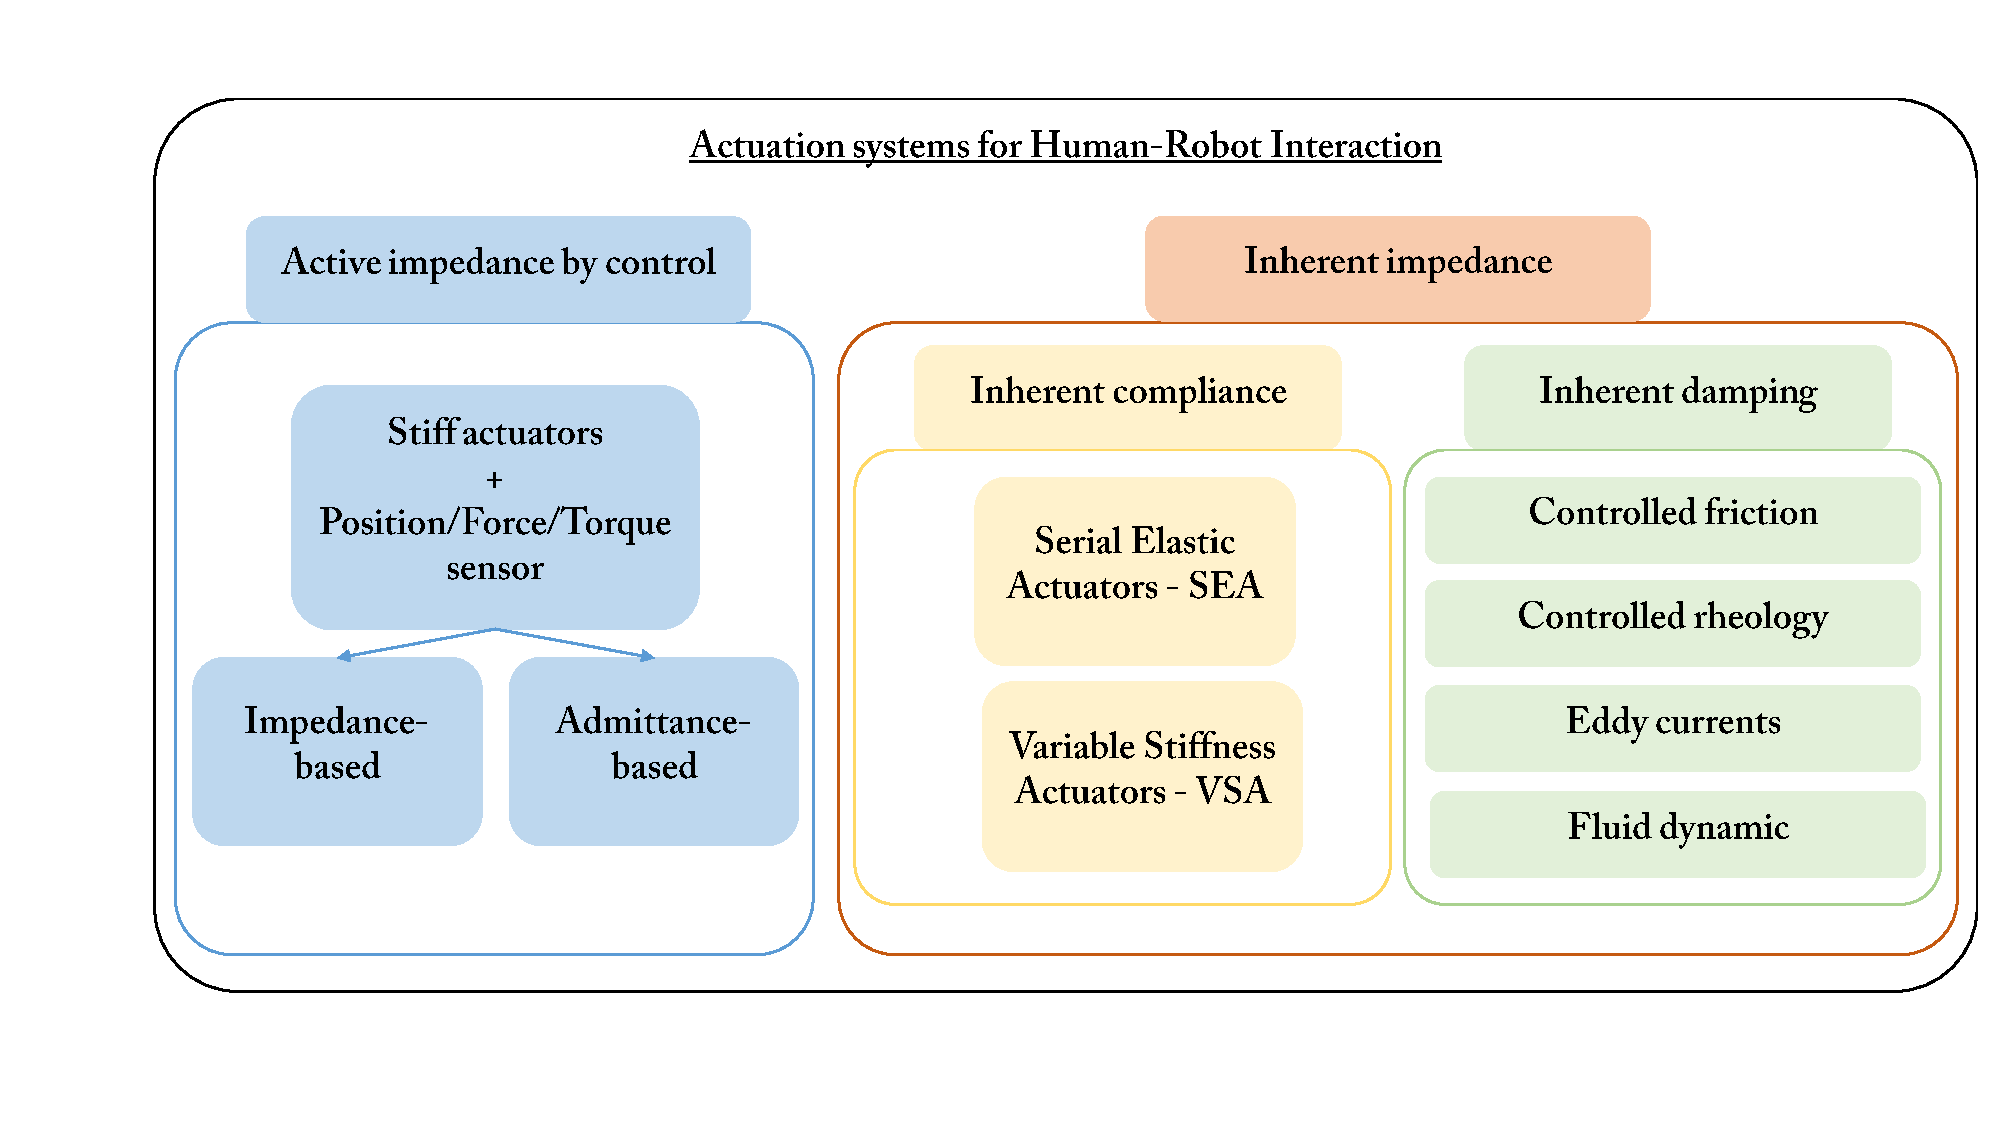
\includegraphics[width=1 \columnwidth]{actuators}
	\def\svgwidth{1\columnwidth}
	\begin{footnotesize}
		\input{imgRevised/SoA.pdf_tex}
	\end{footnotesize}
	\caption{Schema of variable impedance actuation systems for human-robot interaction. The impedance can be simulated and  actively changed by control (this relies on position and torque sensors) or can be an inherent mechanical property of the actuator. In the latter case the mechanical stiffness can be a fixed value (SEA) or can be adjusted (VSA), and the damping can be controlled.}
	\label{fig:exosActuators}
\end{figure}
%
\par In {\em  inherent compliance } actuators an electric motor is coupled with a spring with fixed (Series Elastic Actuator - SEA) or variable stiffness (Variable Stiffness Actuators - VSA), based on the principle that  adding a series elastic element reduces the peak power demand to the motor. {\em Inherent damping } actuators are based on the control of the friction by means of eddy currents, controlled rheology or fluid dynamics. 
%Recently double actuation architectures have been developed for variable impedance actuators	\cite{tagliamonte2012double}, coupling a stiff motor in parallel with an elastic element (Parallel Elastic Actuators - PEA).  Both SEA and VSA have been implemented in exoskeleton as for example in Lopes \cite{veneman2007design}, an exoskeleton for the gait assistance that is based on SEA actuation, or in NEUROexos elbow exoskeleton \cite{vitiello2013neuroexos} that is based on VSA and in ALTACRO locomotion exoskeleton \cite{cherelle2010maccepa} that introduces a Mechanically Adjustable Compliance and Controllable Equilibrium Position Actuator (MACCEPA).
%. 
% 

%Recently double actuation architectures have been developed for variable impedance actuators	\cite{tagliamonte2012double}, coupling a stiff motor in parallel with an elastic element (Parallel Elastic Actuators - PEA).  
Both SEA and VSA have been implemented in exoskeleton as for example in Lopes \cite{veneman2007design},  in NEUROexos elbow exoskeleton \cite{vitiello2013neuroexos}and  ALTACRO locomotion exoskeleton \cite{cherelle2010maccepa}.

All the variable impedance actuators have the advantage of absorbing impacts and SEA and VSA % (inherent compliance) 
can eventually mechanically store energy during passive phases and release it in active phases of the movement cycle.  VSAs generally use two motors which increases the size, weight and complexity of the actuator in comparison with an SEA \cite{wolf2011dlr}.

\par On the other side, {\em active impedance by control}  actuators are composed of electric motors coupled with a transmission/reduction system; they can be classified
according to the backdrivability and sensing system. Force controlled actuators implement a force/torque sensor
at the joint level and can achieve impedance behavior by closed-loop control.
In general traditional actuators with no elastic or damping elements can be lighter and more compact
than passive variable impedance actuators, but their time response and dynamic bandwidth is limited by control and electrical properties of actuators, such as maximum velocity of electrical motor.
%
%The actuation system influences the control design: active exoskeletons can be classified as impedance based design (open-loop impedance control \cite{frisoli2009force} and impedance control with force feedback) or admittance-based design (admittance control with position feedback) \cite{carignan2000closed}.
%
%Open-loop impedance control exoskeletons rely on lightweight designs with joint-delocated motors and backdrivable mechanical solutions, typically implemented making use of tendon transmissions \cite{frisoli2009force}, \cite{perry2007upper}; the most challenging limitations are the friction effects due to the transmission system, that can be compensated only by means of feed-forward compensation based on approximate models, the complexity of the transmission and the difficulty to be mechanically configured in a bilateral configuration, working both for left and right arm. 
%On the other side admittance-based design requires force sensing and can achieve higher stiffness values, but relies on the adopted control for canceling system dynamics and inertia.
%Exoskeleton with a single force/torque sensor localization, such as one torque sensor at the exoskeleton elbow joint and a six-axis force/torque sensor at the exoskeleton handle \cite{carignan2008controlling} or shoulder \cite{nef2007armin}, can accurately regulate interaction forces at the exoskeleton terminal link (i.e. the handle) only.
%Lightweight robots with joint torque sensors \cite{albu2007dlr} allow for multi-contact force/torque control (i.e. the regulation of interaction force/torques at multiple points distributed over multiple links).
%
%
%The correct estimation of interaction force between human and exoskeleton in admittance designs requires control approaches that compensate for friction, inertial and gravity properties of the exoskeleton mechanical structure, but  a complete cancellation of these effects is  difficult to achieve.
%

%
%\begin{figure}[htb]
%	\centering
%	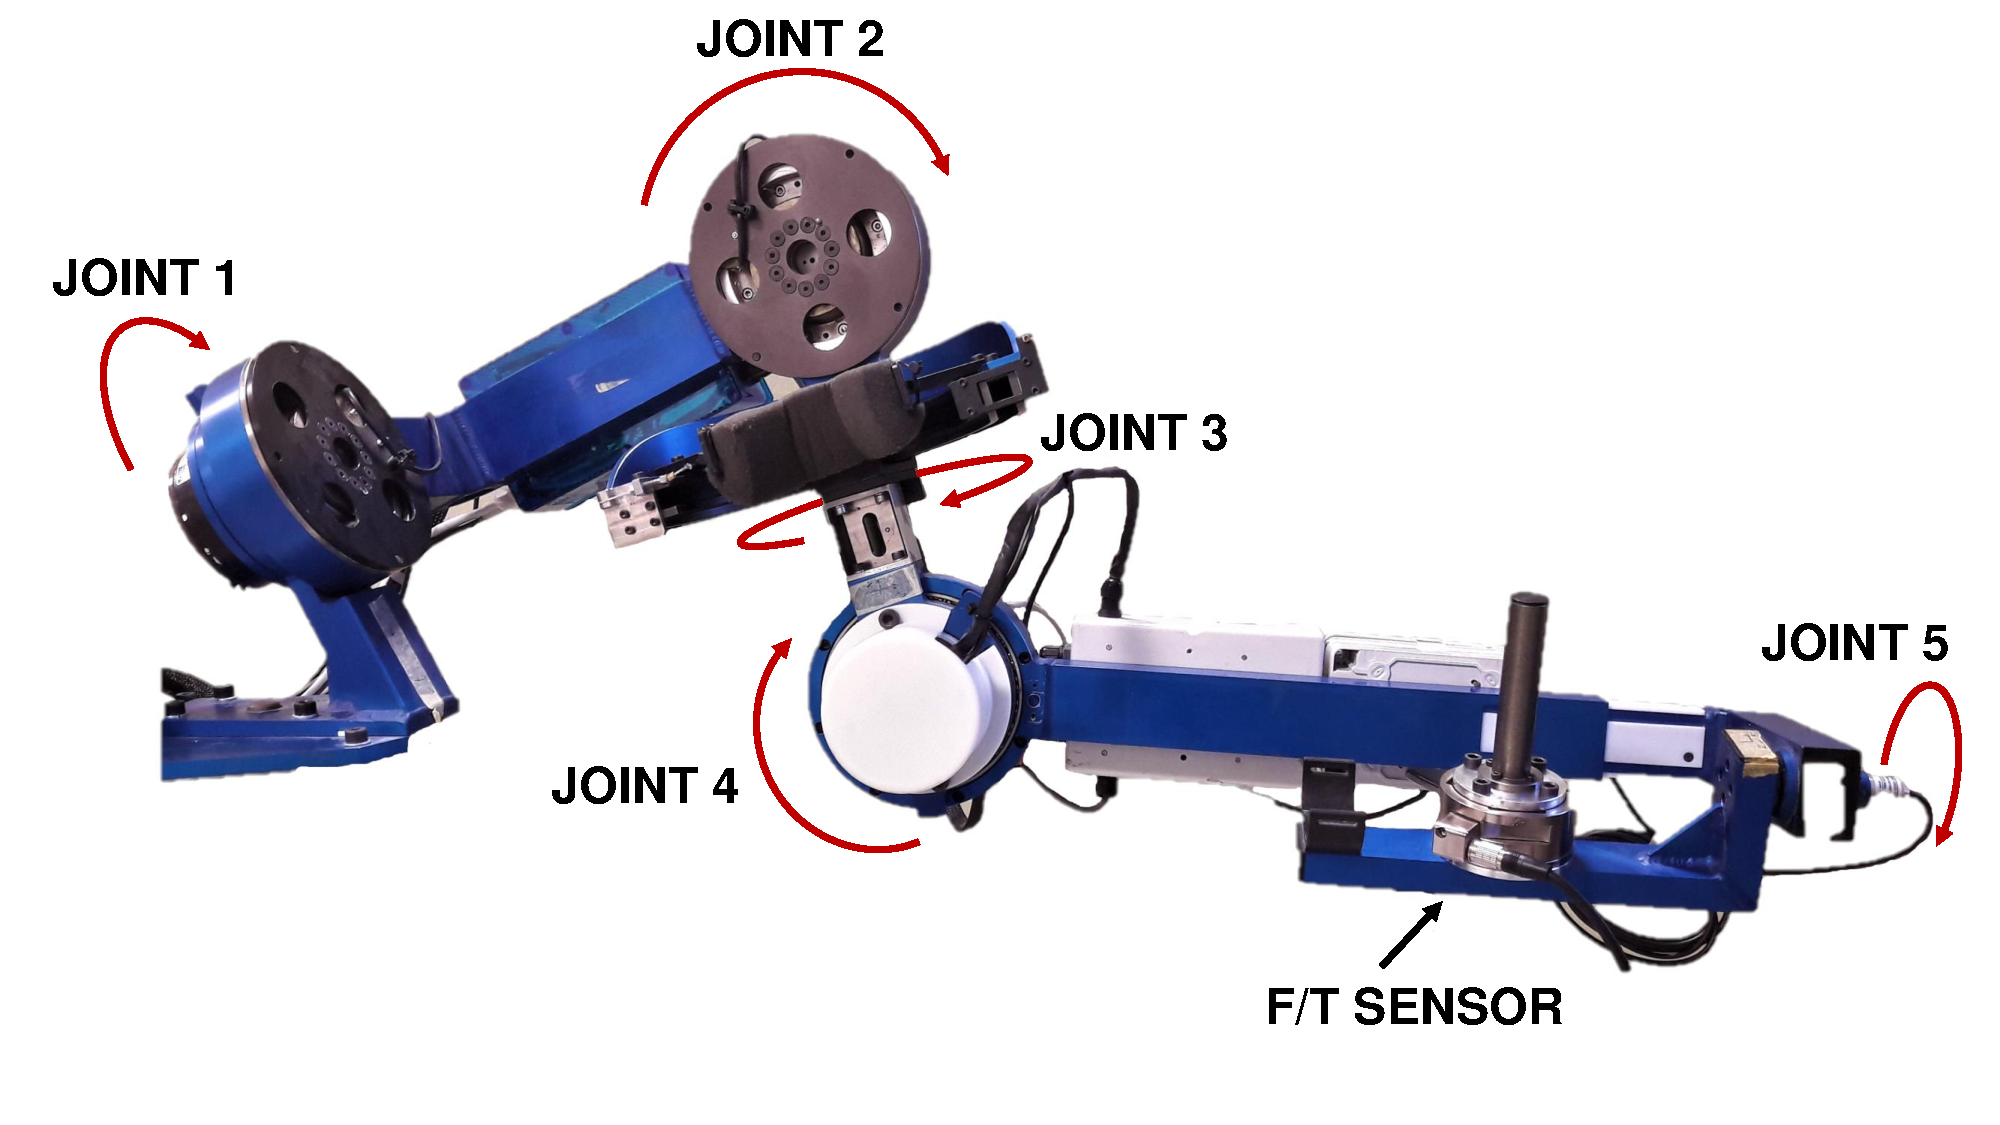
\includegraphics[width=0.95\columnwidth]{RehabDescription} 
%	\hldoing{insert here SoA transparency and issues}
%	\caption{The Rehab-Exos. It is a 5 DOF upper-limb exoskeleton  with 4 actuated joints. The joints $J_1$, $J_2$ and $J_4$ share the same characteristics: high reduction ratio (100:1) by means of harmonic drive, embedded torque sensor and maximum actuation torque of 150 \ Nm. The joint $J_3$ is composed by a semi-circular guide actuated by a DC motor through tendon transmission. Joint $J_5$ is passive and the exoskeleton is equipped of a force/torque sensor at the end-effector that is used for evaluation purposes.}
%	\label{fig:rehabexos1} 
%\end{figure}
%
\par Solutions based on joint torque sensor have been proposed in the last years mostly for example in  lower limb exoskeletons  \cite{kim2015design,aguirre2011design,hwang2015method}. 
%In  \cite{kim2015design} \cite{kim2015design,aguirre2011design,hwang2015method} and in \cite{aguirre2011design} two knee exoskeletons based on joint torque sensor were presented; the latter exoskeleton implements an admittance control based on the torque sensor readings. In \cite{hwang2015method} the torque sensor for a lower limb exoskeleton allows it to accurately estimate the human muscular torque that were exerted during the human-robot interaction. 
The advantage of joint torque sensor based solutions is their compactness and robustness, but when the torque sensor is embedded in the joint it is sensitive to the link inertia in addition to the human interaction torques, thus affecting the system {\em transparency}. A mechanical solution is presented in \cite{zanotto2013improving} where the transparency of a lower-limb exoskeleton has been improved by positioning the force/torque sensor on the supporting cuffs, that is at the interaction point between the human leg and the exoskeleton.
%%%%%%%%%COMMENTED BY ANTONIO IN SECOND REVISION
%%\par Even if SEA and VSA are less compact then traditional actuators, for example \cite{cestari2014ares} \hldoing{not clear here} proposed a solution based on a VSA for an exoskeleton of the leg that reduced the lateral size and integrates a torque sensor based on spring's deflection reads.
 Sensors used to measure these deflections are generally encoders \cite{dos2017design} and potentiometers \cite{junior2016series}; the latter usually require custom mechanical supports to avoid errors related with its sensitivity to misalignments.
While the deflection based force estimation becomes a most widely utilized method for the SEAs and VSAs and performs fidelity force control performance in various robotic applications, there are still difficulties because of the practical issues such as spring deflection measurement error or noise of the encoder signal \cite{lee2018integrated}. These factors have much negative impact on SEA with high stiffness. In \cite{leal2018polymer}, for example, a polymer optical fiber has been mounted on the torsional spring of a SEA to read angles and torques in a more accurate way without considerably enlarging the size of the actuator at the cost of a more specific system electronics.
\par Thus, the adoption of inherent compliant actuation systems rather than achieving compliance by control  is not a trivial choice and it depends on the desired mechanical features and is the result of a trade-off among compactness, weight, simplicity, costs, safety, efficiency.
A good trade-off that prefer compactness, simplicity and uses just one motor is an active impedance by closed-loop control  system that  an elastic component to transmit and to measure axial torques at the same time.


%, extending our previously work presented in \cite{solazzi2014interaction}
\par 
Based on the above, in this paper 
%we address the issue of  collaborative robot behavior,
we introduce the design and the experimental characterization of the Rehab-Exos, an upper limb exoskeleton endowed with  joint torque actuators, based on  joint torque sensors and high reduction ratio, and the design of an  interaction joint torque controller that maximizes both  {\em transparency } and  quality of {\em haptic rendering}.

%The overall control design was optimized and experimentally verified to compare the obseved performance  with two other interaction joint torque architecture used as benchmarking.

%The Rehab-Exos allows to obtain a physical interaction characterized by good {\em transparency } and  quality of {\em haptic rendering}, it is capable to exert a wide range of forces and at the same time it exhibits high position accuracy due to high gear reduction ratio.

\par In particular, to improve transparency we propose a new interaction state-feedback torque controller (JTFC1) that takes into account the multi-dof non linear system dynamics and provides a compensation of other non-linear effects, such as friction and gravity components, to achieve an accurate estimation of human interaction force.
This is accomplished by a single joint optimum observer that ensures joint torque tracking, while a centralized controller estimates and compensates for the dynamics of the whole system. 
%Moreover, we have evaluated the effect of dynamic compensation on system transparency highlighting good results.
\par To validate the proposed controller as well as the chosen mechanical architecture, the full-state feedback controller was  compared with two alternative controllers,  a  feedback controller (JTFC2) and a passivity-based feedback controller (JTFC3), in two tasks: the zero desired force tracking ({\em transparency}) and the contact with a virtual stiff wall ({\em haptic rendering}). 
The {\em transparency} benchmarking test among the 3 controllers was performed experimentally with 10 subjects and two different reference velocities, according to the evaluation procedure already tested in \cite{just2018exoskeleton}, in order to achieve comparable benchmark results.

As far as haptic rendering, the stability behavior and quality of force rendering of the proposed controller was assessed through a virtual wall simulation implemented with increasing  stiffness values and  compared it with the other two  benchmark controllers.
In  both experimental conditions,  the proposed joint torque controller allows it to achieve higher performance both in term of transparency and haptic rendering, demonstrating how an active impedance by control  can reach optimal performance if suitable state feedback is employed.
%Results reward the chosen mechanical and control strategy as presented in the last part of this paper.


%\par The first part of the paper widely treats the critical issue due to the use of a torque sensor embedded in the joint and in particular the sensitivity to non-axial load has been studied. Then, in the second part the joint model and the control technique are presented.

\par This paper is structured as follows: Section \ref{sec:systemDesign} presents the design of the Rehab-Exos with a particular focus on the strain gauge-based torque sensor design and issues. Section \ref{Single joint model} provides a mathematical model of the single joint whereas in the Section \ref{Full dynamics model} the full dynamics model of the Rehab-Exos is described. Section \ref{sec:Full_state_feedback_controllers} explains the proposed full state feedback controller and recalls two benchmark torque controllers already known in literature. Section \ref{sec:experimentsResults} presents the experiments and the obtained results.
Finally, discussions and conclusions are addressed in Sections \ref{sec:discussion} and \ref{sec:conclusion} respectively.  

%
%Active exoskeleton systems are robotic devices that can be worn on the user's body, implying that they should satisfy requirements of safety and better compliance.
%After the Fukushima event in Japan, the application of these human-robot interfaces in the area of rescue robotics and teleoperation has became an emerging field of research,
%for which the development of upper limb active exoskeletons with dexterous manipulation abilities has become a hot topic of research.
%Another relevant sector of application of active exoskeletons is represented by neuro-motor rehabilitation post-stroke \cite{lo2012exoskeleton}, where different prototypes and commercial solutions have been recently proposed.
%
%
%While the general rationale for the design of high performance haptic interfaces are the satisfaction of the requirements of high force fidelity, transparency
%and backdrivability, specific issues need to be addressed in exoskeleton design in terms of safety, kinematics and ....
%
%For what concerns, upper limb exoskeletons, we should consider:
%\begin{description}
%\item[User requirements] Safety: the structure is always in close contact with the user
%\item[Design issues, kinematics, mechanical design]
%The kinematics should be adjusted to user arm, Possibility of adjusting the size of the system to avoid internal forces
%Complexity of shoulder motion, Non periodicity of upper limb movement compared to lower limb, Intrinsic 3D spatial motion Both left and right arm schemes should be implementable
%\item[Design issues, control] Low inertia should be achieved, possibility of employing force sensors, Remote vs. local actuation, High forces required (no gravity cancellation provided by support elements e.g., support plans)
%\end{description}
%
%%In SSSA there is a consolidated experience in the design and development of new exoskeleton systems \cite{frisoli2005new}, as shown in figure~\ref{fig:exos@SSSA}.
%
%%%%%%%%%%%%%%%%%%%%%%%%%%%%%%%%%%%%%%%%%%%%%%%%%%%%%%%%%%%%%%%%%%%%%%%%%%%%%%%%%%%%%%%%%%%%%%%%%%%%%%%%%%%%%%%%%%%%
%%%%%%%%%%%%%%%%%%%%%%%%%%%%%%%%%%%%%%%%%%%%%%%%%%%%%%%%%%%%%%%%%%%%%%%%%%%%%%%%%%%%%%%%%%%%%%%%%%%%%%%%%%%%%%%%%%%%
%%%%%%%%%%%%%%%%%%%%%%%%%%%%%%%%%%%%%%%%%%%%%%%%%%%%%%%%%%%%%%%%%%%%%%%%%%%%%%%%%%%%%%%%%%%%%%%%%%%%%%%%%%%%%%%%%%%%
%%%%%%%%%%%%%%%%%%%%%%%%%%%%%%%%%%%%%%%%%%%%%%%%%%%%%%%%%%%%%%%%%%%%%%%%%%%%%%%%%%%%%%%%%%%%%%%%%%%%%%%%%%%%%%%%%%%%

